\documentclass[11pt]{article}
\usepackage{graphicx}
\usepackage{float}
\usepackage{listings}
\usepackage{caption}
\usepackage{amsmath}
\usepackage{listings}
\usepackage{xcolor}
\usepackage[top = 0.7in,bottom = 1in, left = 0.8in, right = 0.8in]{geometry} 

%New colors defined below
\definecolor{codegreen}{rgb}{0,0.6,0}
\definecolor{codegray}{rgb}{0.5,0.5,0.5}
\definecolor{codepurple}{rgb}{0.58,0,0.82}
\definecolor{backcolour}{rgb}{0.95,0.95,0.92}

%Code listing style named "mystyle"
\lstdefinestyle{mystyle}{
  backgroundcolor=\color{backcolour},   commentstyle=\color{codegreen},
  keywordstyle=\color{magenta},
  numberstyle=\tiny\color{codegray},
  stringstyle=\color{codepurple},
  basicstyle=\ttfamily\footnotesize,
  breakatwhitespace=false,         
  breaklines=true,                 
  captionpos=b,                    
  keepspaces=true,                 
  numbers=left,                    
  numbersep=5pt,                  
  showspaces=false,                
  showstringspaces=false,
  showtabs=false,                  
  tabsize=2
} 
\lstset{style=mystyle}

\title{\textbf{CS747 : Programming Assignment 2}}
\author{\textbf{Adityaya Dhande}   \hspace{8mm} \textbf{210070005}}
\begin{document}
\maketitle
\section*{Task 1}

\subsection*{Value Iteration}
\begin{lstlisting}[language=Python]      
def B_star(self, Vt):
    T = self.T 
    R = self.R 
    gamma = self.gamma        
    avals = np.sum(T * (R + gamma * Vt), axis=2)
    V = np.max(avals, axis=1)
    Pi = np.argmax(avals, axis=1)
    return V, Pi

def vi(self):
    tol = 1e-7
    V_old = np.zeros(self.numStates)
    V_new, Pi = self.B_star(V_old)
    count = 0
    delta = np.linalg.norm(V_new - V_old)
    while delta > tol :
        V_old = V_new
        V_new, Pi = self.B_star(V_old)
        count += 1
        delta = np.linalg.norm(V_new - V_old)
    return V_new, Pi
\end{lstlisting}
\noindent
\textbf{Code explanation :} The function \texttt{B\_star} is the Bellman optimality 
operator, which takes a Value function $V_t$ and returns $B^* (V_t)$ as $$ 
(B^*(V_t))(s) = \max_{a \in A} \sum\limits_{s' \in S} T(s, a, s')\{R(s, a, s') + \gamma V_t(s')\}
$$ I vectorised the 
code for this function by using \texttt{numpy} arrays (lines 5, 6 and 7 axis = 0 corresponds
to $s$, axis = 1 corresponds to $a$ and axis = 2 corresponds to $s'$). It also returns a 
policy consisting on an action for each state which gives the maximum Value function. 
The function \texttt{vi} first initialises a value function which is 0 for all the states and then
iteratively applies the Bellman optimality operator on it till the $L_2$ norm of the difference between the successive 
value functions becomes less than $10^{-7}$. It returns this value function and policy which are close to the
optimal value function and optimal policy respectively. 
    \newpage
   \subsection*{Linear Programming}

\begin{lstlisting}[language=Python]      
def evaluate_value(self, Pi):
    b = np.zeros(self.numStates)
    A = np.zeros((self.numStates, self.numStates))
    for i in range(self.numStates):
        b[i] = -np.sum(self.T[i, Pi[i], :] * self.R[i, Pi[i], :])
        A[i, :] = self.T[i, Pi[i], :] * self.gamma
        A[i, i] -= 1
    V_new = np.linalg.solve(A, b)
    return V_new

def action_value(self, s, a, V):
    T_sa = self.T[s, a, :]
    R_sa = self.R[s, a, :]
    q = np.sum(T_sa * (R_sa + self.gamma * V))
    return q

def get_pi_star(self, V):
    Pi = np.zeros(self.numStates, dtype=np.int32)
    for i in range(self.numStates):
        avals = np.zeros(self.numActions)
        for j in range(self.numActions):
            avals[j] = self.action_value(i, j, V)
        Pi[i] = np.argmax(avals)
    return Pi

def lp(self):
    prob = pulp.LpProblem('OptimalPolicyFinder', pulp.LpMaximize)
    variables = [pulp.LpVariable('V' + str(i)) for i in range(self.numStates)]
    cost = -pulp.lpSum(variables)
    prob += cost
    for i in range(self.numStates):
        for j in range(self.numActions):
            sum1 = np.sum(self.T[i, j, :] * self.R[i, j, :])
            string = pulp.lpSum(self.T[i, j, k] * self.gamma * variables[k] for k in range(self.numStates)) + sum1
            prob += variables[i] >= string
    prob.solve(pulp.PULP_CBC_CMD(msg=0))
    V_dict = {v.name[1:]: v.varValue for v in prob.variables()}
    V_star = np.array([V_dict[str(i)] for i in range(self.numStates)])
    return V_star, self.get_pi_star(V_star)
\end{lstlisting}
    \noindent
    \textbf{Code explanation :} The function \texttt{evaluate\_value} evaluates the
    value function for a given policy. I chose to use the method of solving the Bellman
    equations for this purpose as it is more accurate when compared to the iterative method
    of applying the Bellman operator. The function \texttt{action\_value} evaluates the 
    action value of an action for a given state and value function. The function \texttt{get\_pi\_star}
    returns the optimal policy when the argument passed is the optimal value function as for
    each state it returns the action with the maximum action value. The function \texttt{lp}
    forms the constraints using the value function as ``n variables'' (a value for each state) and 
    also defines the objective function as discussed in class. It then uses the PuLP solver to 
    solve the linear programming problem and obtain the optimal value function, and also
    calculates the optimal policy by invoking \texttt{get\_pi\_star}.
    \\ \texttt{V\_dict} stores the mapping from the value function of the states to the 
    PuLP variables
\newpage
\subsection*{Howard's Policy Iteration}
 

 \begin{lstlisting}[language=Python]      
def improving_actions(self, V_pi, s):
    action_values = np.array([self.action_value(s, i, V_pi) for i in range(self.numActions)])
    IA = np.where(action_values - V_pi[s] > 1e-9)[0]
    return IA.tolist()

def improvable_states(self, Pi):
    V_pi = self.evaluate_value(Pi)
    improving_actions_all = [self.improving_actions(V_pi, i) for i in range(self.numStates)]
    IS_indices = np.where(np.array([len(ia) > 0 for ia in improving_actions_all]))[0]
    IS = {i: improving_actions_all[i] for i in IS_indices}
    return IS


def hpi(self):
    Pi = np.zeros(self.numStates, dtype=np.int32)
    IS = self.improvable_states(Pi)
    
    while IS:
        improvable_states_indices = list(IS.keys())
        random_actions = np.array([random.choice(IS[i]) for i in improvable_states_indices])
        Pi[improvable_states_indices] = random_actions
        IS = self.improvable_states(Pi)
    
    Vpi = self.evaluate_value(Pi)
    return Vpi, Pi      
\end{lstlisting}
\noindent
    \textbf{Code explanation :} The function \texttt{improving\_actions} returns all the actions
    that have an action value greater than the given value function for a given state. The function \texttt{improvable\_states}
    returns all the states which have one or more improving actions. The function \texttt{hpi}
    initialises a policy which chooses action 0 for all states and then finds all the improvable states and the corresponding improving
    actions and picks an improving action uniformly for all the improvable states. It does this
    iteratively till the number of improvable states becomes zero. 
    \\[2\baselineskip] Value iteration was easily vectorisable as compared to linear programming
    and Howard's policy iteration.
    \newpage
\section*{Task 2}
\subsection*{Formulation of the MDP}
I did the following to formulate the MDP :
\begin{enumerate}
    \item The total number of states possible are $16 \times 16 \times 16 \times 2 + 2 = 8194$, where
    8192 states are the permutations of positions of B1, B2 and R on the $4\times4$ grid and the possession of ball. The remaining 
    2 states are terminal states, one for a WIN and one for a LOSS. 
    \item For each of the 8194 states there are 10 actions possible and we need to assign the transition probabilities to all these actions in each state. To begin with I assigned all the transitions a 0 probability and then changed all the non-zero transition probabilities.
    \item The states 0 to 8191 are, in the same order, the ones in the opponent policy file and 8192 is the state for a LOSS and 8193 for a WIN. So
    the transition from state 8192 on taking any action is 0 for all states and 1 for 8192. Same holds for the state 8193.
    \item Now we iterate through the remaining states(0 to 8191) and the 10 actions for each state. For each of these states we obtain the opponent's policy
    and compute the possible positions of R for a given state. For each of these positions of R, I then evaluated the probabilities
    of winning, losing, moving, passing and getting tackled as described. 
    \item This probability should be multiplied with the probability that R moves to that particular position. I created a dictionary which contains a mapping from player positions and possession to the state indices, which I used
    to compute the new state that the transition occurs to, and increased the array of transition probabilities at that index by the computed probability. I also populated the probability of a LOSS or WIN. 
    \item I set the reward function to be zero for all transitions, except for when you transition to the WIN state, for which the reward is 1.
\end{enumerate}
\subsection*{Analysis}
\begin{figure}[H]
    \begin{center} 
        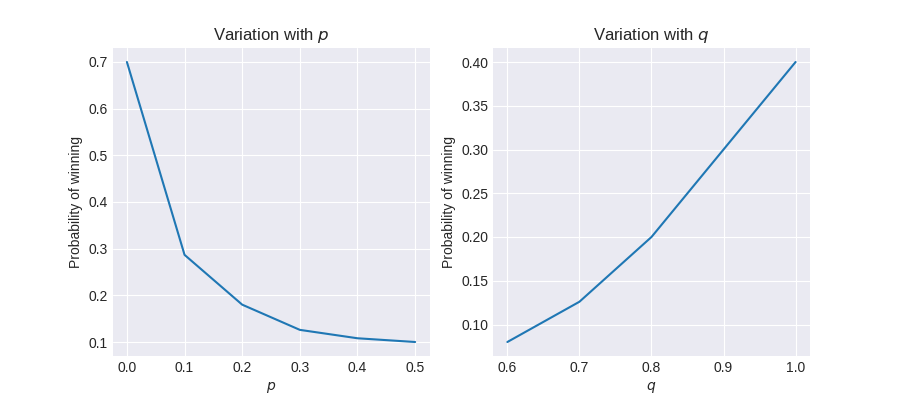
\includegraphics[width=1\textwidth]{../images/plot3.png}
        \caption*{Variation in probability of winning with $p$ and $q$ for starting position = [05, 09, 08, 1]}
    \end{center}
 \end{figure}
The variation of probability of winning with $p$ and $q$ matches with out intuition as 
for lower values of $p$, the probability that a moving player loses possession is low and also the probability
that they get tackled is low. For high values of $q$ the probability that a pass is successful is high 
and the probability of scoring a goal on shooting is also high. Thus probability of winning show decrease with increase in $p$
and increase with increase in $q$ intuitively.
\noindent
\\
\\
I also evaluated the probabilities of winning from a starting position of [05, 09, 08, 1]
for the same values of $p = 0.25$ and $q = 0.75$ but for different opponent policies. 
The results were as follows :
\begin{itemize}
    \item Greedy defense : 0.175
    \item Park the bus : 0.0875
    \item Random policy : 0.1552
\end{itemize}
This indicates that Greedy defense is the best policy for the starting position of [05, 09, 08, 1]
\end{document}
 